\documentclass{beamer}
\usepackage{graphicx}
\usepackage{tikz}
\usepackage[most]{tcolorbox}


%THEME and COLORTHEME
\usetheme{Madrid}

% \usetheme{Berkeley}
% \usetheme{Copenhagen}

% \usecolortheme{beaver}
% \usecolortheme{beetle}
% \usecolortheme{seahorse}
% \usecolortheme{wolverine}

%DEMO TITLEPAGE
%Information to be included in the title page:
% \title{Title}
% \author{Author}
% \institute{Institute}
% \date{\today}

%FIXING TITLEPAGE
\title{\textbf{Strongly Connected Components}}

% \subtitle{An Introduction}

\author[Asif \and Fahim]
{\large {\textbf{Md. Asif Haider (1805112)}} \\ \large{\textbf{K.M Fahim Shahriyar (1805113)}}}

%\author{A.~B \and X.~Y}

\institute[BUET]
{
 \large {Department of Computer Science and Engineering\\
  Bangladesh University of Engineering and Technology}
}

\date{\today}

\logo{\includegraphics[height=1cm]{logo.png}}

% PLACING ToC AT THE BEGINNING OF EACH SECTION
% \AtBeginSection[]
% {
%   \begin{frame}
%     \frametitle{Table of Contents}
%     \tableofcontents[currentsection]
%   \end{frame}
% }

\begin{document}

\frame{\titlepage}

\tikzstyle{Node}=[circle,draw=blue!50,fill=blue!20,ultra thick]
\tikzstyle{Node_2}=[circle,draw=orange!50,fill=orange!20,ultra thick]

\begin{frame}{Strong Connectivity}

\begin{alertblock}{Strongly Connected Graph}
 A graph G(V,E) is called Strongly Connected Graph if every pair of nodes is \textbf{mutually reachable}
\end{alertblock}

\pause
\begin{block}{Remark}
 Strong Connectivity is the property of \alert{\textbf{Directed Graph}}
\end{block}
    
\end{frame}


\begin{frame}{Example of Strong Connectivity}

\begin{figure}
    \centering

\begin{tikzpicture}

\node[Node_2] (B_Node) {B};
\node[Node_2] (C_Node) [right of=B_Node,xshift = 10mm] {C};
\node[Node_2] (A_Node) [above of=E_Node,yshift = 10mm, xshift = 10mm] {A};

\draw [->,ultra thick] (A_Node) to (B_Node);
\draw [->,ultra thick] (B_Node) to (C_Node);
\draw [->,ultra thick] (C_Node) to (A_Node);


\end{tikzpicture}

    \caption{Strongly Connected Graph}
   
\end{figure}

\pause
\begin{tcolorbox}[colback=red!5!white,colframe=red!75!black]
\centering
  In this graph every nodes are mutually reachable
\end{tcolorbox}


    
\end{frame}



\begin{frame}{Example of Strong Connectivity(Contd.)}

\begin{figure}
    \centering

\begin{tikzpicture}

\node[Node_2] (B_Node) {B};
\node[Node_2] (C_Node) [right of=B_Node,xshift = 10mm] {C};
\node[Node_2] (A_Node) [above of=E_Node,yshift = 10mm,xshift = 10mm] {A};

\draw [->,ultra thick] (A_Node) to (B_Node);
\draw [->,ultra thick] (B_Node) to (C_Node);
\draw [->,ultra thick] (A_Node) to (C_Node);

\draw<2-> [black][dashed] (1,0) ellipse (2 and 0.8) ;

\end{tikzpicture}

    \caption{Not Strongly Connected Graph}
   
\end{figure}

\pause

\begin{tcolorbox}[colback=red!5!white,colframe=red!75!black]
\centering
  In this graph from \alert{\textbf{B}} only \alert{\textbf{C}} is reachable.
  \alert{\textbf{A}} is not reachable
\end{tcolorbox}


    
\end{frame}

\begin{frame}{Strongly Connected Component}

\begin{alertblock}{Strongly Connected Components}
Strongly Connected Components of a directed graph are the subgraphs which are  \alert{\textbf{individually strongly connected}}
\end{alertblock}
    
\end{frame}

\begin{frame}{Example of Strongly Connected Components}


\begin{figure}
    \centering

\begin{tikzpicture}

\node[Node] (A_Node) {A};
\node[Node] (B_Node) [below of=A_Node,yshift = -10mm] {B};
\node[Node] (C_Node) [right of=A_Node,xshift = 10mm] {C};
\node[Node] (D_Node) [below of=C_Node,yshift = -10mm] {D};
\node[Node] (E_Node) [right of=D_Node,xshift = 10mm] {E};
\node[Node] (F_Node) [right of=E_Node,xshift = 10mm] {F};
\node[Node] (H_Node) [right of=F_Node,xshift = 10mm] {H};
\node[Node] (G_Node) [above of=E_Node,yshift = 10mm,xshift = 10mm] {G};

\draw [->,ultra thick] (A_Node) to (C_Node);
\draw [->,ultra thick] (B_Node) to (A_Node);
\draw [->,ultra thick] (D_Node) to (B_Node);
\draw [->,ultra thick] (C_Node) to (D_Node);
\draw [->,ultra thick] (D_Node) to (E_Node);
\draw [->,ultra thick] (F_Node) to (E_Node);
\draw [->,ultra thick] (F_Node) to (H_Node);
\draw [->,ultra thick] (E_Node) to (G_Node);
\draw [->,ultra thick] (G_Node) to (F_Node);


\end{tikzpicture}

    \caption{A Directed Graph}
   
\end{figure}


    
\end{frame}


\begin{frame}{Example of Strongly Connected Components (Continued)}



\begin{columns}
    

\column{0.6\textwidth}
\centering
Given Graph
\begin{figure}[t]
\begin{tikzpicture}

\node[Node] (A_Node) {A};
\node[Node] (B_Node) [below of=A_Node,yshift = -5mm] {B};
\node[Node] (C_Node) [right of=A_Node,xshift = 5mm] {C};
\node[Node] (D_Node) [below of=C_Node,yshift = -5mm] {D};
\node[Node] (E_Node) [right of=D_Node,xshift = 5mm] {E};
\node[Node] (F_Node) [right of=E_Node,xshift = 5mm] {F};
\node[Node] (H_Node) [right of=F_Node,xshift = 5mm] {H};
\node[Node] (G_Node) [above of=E_Node,yshift = 5mm,xshift = 5mm] {G};

\draw [->,ultra thick] (A_Node) to (C_Node);
\draw [->,ultra thick] (B_Node) to (A_Node);
\draw [->,ultra thick] (D_Node) to (B_Node);
\draw [->,ultra thick] (C_Node) to (D_Node);
\draw [->,ultra thick] (D_Node) to (E_Node);
\draw [->,ultra thick] (F_Node) to (E_Node);
\draw [->,ultra thick] (F_Node) to (H_Node);
\draw [->,ultra thick] (E_Node) to (G_Node);
\draw [->,ultra thick] (G_Node) to (F_Node);


    \draw <2-3> [blue][dashed,ultra thick] (0.75,-0.8) circle [radius=1.55];
    \draw <4-5> [blue][dashed,ultra thick] (3.65,-0.8) circle [radius=1.55];
     \draw <6-7> [blue][dashed,ultra thick] (6.0,-1.5) circle [radius=0.8];
     
\end{tikzpicture}

\end{figure}

  
\column<3->{0.4\textwidth}

\centering
Strongly Connected Components


\begin{figure}[t]
\begin{tikzpicture}

\node<3->[Node] (A_Node) {A};
\node<3->[Node] (B_Node) [below of=A_Node,yshift = -5mm] {B};
\node<3->[Node] (C_Node) [right of=A_Node,xshift = 5mm] {C};
\node<3->[Node] (D_Node) [below of=C_Node,yshift = -5mm] {D};


\draw<3-> [->,ultra thick] (A_Node) to (C_Node);
\draw<3-> [->,ultra thick] (B_Node) to (A_Node);
\draw<3-> [->,ultra thick] (D_Node) to (B_Node);
\draw<3-> [->,ultra thick] (C_Node) to (D_Node);

\end{tikzpicture}
\end{figure}


\begin{figure}[t]

\begin{tikzpicture}

\node<5->[Node] (E_Node) {E};
\node<5->[Node] (F_Node) [right of=E_Node,xshift = 5mm] {F};
\node<5->[Node] (G_Node) [above of=E_Node,yshift = 5mm,xshift = 5mm] {G};

\draw<5-> [->,ultra thick] (F_Node) to (E_Node);
\draw<5-> [->,ultra thick] (E_Node) to (G_Node);
\draw<5-> [->,ultra thick] (G_Node) to (F_Node);

\end{tikzpicture}
\end{figure}


\begin{figure}[t]

\begin{tikzpicture}

\node<7->[Node] (H_Node) {H};


\end{tikzpicture}
\end{figure}

 \end{columns}  



\end{frame}

\begin{frame}{Strongly Connected Components of a Directed Graph }
\centering
Given Graph
\begin{figure}[t]
\begin{tikzpicture}

\node[Node] (A_Node) {A};
\node[Node] (B_Node) [below of=A_Node,yshift = -5mm] {B};
\node[Node] (C_Node) [right of=A_Node,xshift = 5mm] {C};
\node[Node] (D_Node) [below of=C_Node,yshift = -5mm] {D};
\node[Node] (E_Node) [right of=D_Node,xshift = 5mm] {E};
\node[Node] (F_Node) [right of=E_Node,xshift = 5mm] {F};
\node[Node] (H_Node) [right of=F_Node,xshift = 5mm] {H};
\node[Node] (G_Node) [above of=E_Node,yshift = 5mm,xshift = 5mm] {G};

\draw [->,ultra thick] (A_Node) to (C_Node);
\draw [->,ultra thick] (B_Node) to (A_Node);
\draw [->,ultra thick] (D_Node) to (B_Node);
\draw [->,ultra thick] (C_Node) to (D_Node);
\draw [->,ultra thick] (D_Node) to (E_Node);
\draw [->,ultra thick] (F_Node) to (E_Node);
\draw [->,ultra thick] (F_Node) to (H_Node);
\draw [->,ultra thick] (E_Node) to (G_Node);
\draw [->,ultra thick] (G_Node) to (F_Node);



\end{tikzpicture}

\end{figure}
\\
\\
 
\begin{tcolorbox}[enhanced,sharp corners=uphill,
    colback=white!50!white,colframe=blue!25!black,coltext=black,
    fontupper=\bfseries,arc=6mm,boxrule=2mm,boxsep=5mm,
    borderline={0.3mm}{0.3mm}{white}]
 So finally the Strongly Connected Components are : \alert{\{A,B,C,D\},\{E,F,G\},\{H\}}
\end{tcolorbox}
        
 
\end{frame}

\begin{frame}{Finding Strongly Connected Components}

\centering
Given Graph

\begin{figure}[t]
\begin{tikzpicture}

\node[Node] (A_Node) {A};
% \node[Node_2] (A_Node) {A};
\node[Node] (B_Node) [below of=A_Node,yshift = -5mm] {B};
% \node[Node_2] (B_Node) [below of=A_Node,yshift = -5mm] {B};
\node[Node] (C_Node) [right of=A_Node,xshift = 5mm] {C};
% \node[Node_2] (C_Node) [right of=A_Node,xshift = 5mm] {C};
\node[Node] (D_Node) [below of=C_Node,yshift = -5mm] {D};
% \node[Node_2] (D_Node) [below of=C_Node,yshift = -5mm] {D};
\node[Node] (E_Node) [right of=D_Node,xshift = 5mm] {E};
% \node[Node_2] (E_Node) [right of=D_Node,xshift = 5mm] {E};
\node[Node] (F_Node) [right of=E_Node,xshift = 5mm] {F};
% \node[Node_2] (F_Node) [right of=E_Node,xshift = 5mm] {F};
\node[Node] (H_Node) [right of=F_Node,xshift = 5mm] {H};
% \node[Node_2] (H_Node) [right of=F_Node,xshift = 5mm] {H};
\node[Node] (G_Node) [above of=E_Node,yshift = 5mm,xshift = 5mm] {G};
% \node[Node_2] (G_Node) [above of=E_Node,yshift = 5mm,xshift = 5mm] {G};

\draw [->,ultra thick] (A_Node) to (C_Node);
\draw [->,ultra thick] (B_Node) to (A_Node);
\draw [->,ultra thick] (D_Node) to (B_Node);
\draw [->,ultra thick] (C_Node) to (D_Node);
\draw [->,ultra thick] (D_Node) to (E_Node);
\draw [->,ultra thick] (F_Node) to (E_Node);
\draw [->,ultra thick] (F_Node) to (H_Node);
\draw [->,ultra thick] (E_Node) to (G_Node);
\draw [->,ultra thick] (G_Node) to (F_Node);



\end{tikzpicture}

\end{figure}

\begin{itemize}
    \item<1-> \textbf{How to decompose a directed graph into strongly connected components?}
    \pause
    \item<2-> \textbf{The idea is to use \alert{Depth First Search} , but in a tricky way!}
\end{itemize}

\end{frame}



\begin{frame}{Simulation: Kosaraju's Algorithm}

\begin{itemize}
    \item <1-> \textbf{Step 1:} DFS and Topological Sort on the given graph
\end{itemize}

\begin{figure}[t]
\begin{tikzpicture}

\node<1->[Node] (A_Node) {A};
\node<2>[Node_2] (A_Node) {1/};
\node<3->[Node] (A_Node) {1/};
\node<18>[Node_2] (A_Node) {1/16};
\node<19->[Node] (A_Node) {1/16};

\node<1->[Node] (C_Node) [right of=A_Node,xshift = 5mm] {C};
\node<3>[Node_2] (C_Node) [right of=A_Node,xshift = 5mm] {2/};
\node<4->[Node] (C_Node) [right of=A_Node,xshift = 5mm] {2/};
\node<17>[Node_2] (C_Node) [right of=A_Node,xshift = 5mm] {2/15};
\node<18->[Node] (C_Node) [right of=A_Node,xshift = 5mm] {2/15};

\node<1->[Node] (D_Node) [below of=C_Node,yshift = -5mm] {D};
\node<4>[Node_2] (D_Node) [below of=C_Node,yshift = -5mm] {3/};
\node<5->[Node] (D_Node) [below of=C_Node,yshift = -5mm] {3/};
\node<16>[Node_2] (D_Node) [below of=C_Node,yshift = -5mm] {3/14};
\node<17->[Node] (D_Node) [below of=C_Node,yshift = -5mm] {3/14};

\node<1->[Node] (B_Node) [below of=A_Node,yshift = -5mm] {B};
\node<5>[Node_2] (B_Node) [below of=A_Node,yshift = -5mm] {4/};
\node<6->[Node] (B_Node) [below of=A_Node,yshift = -5mm] {4/};
\node<6>[Node_2] (B_Node) [below of=A_Node,yshift = -5mm] {4/5};
\node<7->[Node] (B_Node) [below of=A_Node,yshift = -5mm] {4/5};

\node<1->[Node] (E_Node) [right of=D_Node,xshift = 5mm] {E};
\node<8>[Node_2] (E_Node) [right of=D_Node,xshift = 5mm] {6/};
\node<9->[Node] (E_Node) [right of=D_Node,xshift = 5mm] {6/};
\node<15>[Node_2] (E_Node) [right of=D_Node,xshift = 5mm] {6/13};
\node<16->[Node] (E_Node) [right of=D_Node,xshift = 5mm] {6/13};

\node<1->[Node] (G_Node) [above of=E_Node,yshift = 5mm,xshift = 5mm] {G};
\node<9>[Node_2] (G_Node) [above of=E_Node,yshift = 5mm,xshift = 5mm] {7/};
\node<10->[Node] (G_Node) [above of=E_Node,yshift = 5mm,xshift = 5mm] {7/};
\node<14>[Node_2] (G_Node) [above of=E_Node,yshift = 5mm,xshift = 5mm] {7/12};
\node<15->[Node] (G_Node) [above of=E_Node,yshift = 5mm,xshift = 5mm] {7/12};


\node<1->[Node] (F_Node) [right of=E_Node,xshift = 5mm] {F};
\node<10>[Node_2] (F_Node) [right of=E_Node,xshift = 5mm] {8/};
\node<11->[Node] (F_Node) [right of=E_Node,xshift = 5mm] {8};
\node<13>[Node_2] (F_Node) [right of=E_Node,xshift = 5mm] {8/11};
\node<14->[Node] (F_Node) [right of=E_Node,xshift = 5mm] {8/11};

\node<1->[Node] (H_Node) [right of=F_Node,xshift = 5mm] {H};
\node<11>[Node_2] (H_Node) [right of=F_Node,xshift = 5mm] {9/};
\node<12->[Node] (H_Node) [right of=F_Node,xshift = 5mm] {9/};
\node<12>[Node_2] (H_Node) [right of=F_Node,xshift = 5mm] {9/10};
\node<13->[Node] (H_Node) [right of=F_Node,xshift = 5mm] {9/10};


\draw [->,ultra thick] (A_Node) to (C_Node);
\draw [->,ultra thick] (B_Node) to (A_Node);
\draw [->,ultra thick] (D_Node) to (B_Node);
\draw [->,ultra thick] (C_Node) to (D_Node);
\draw [->,ultra thick] (D_Node) to (E_Node);
\draw [->,ultra thick] (F_Node) to (E_Node);
\draw [->,ultra thick] (F_Node) to (H_Node);
\draw [->,ultra thick] (E_Node) to (G_Node);
\draw [->,ultra thick] (G_Node) to (F_Node);


\end{tikzpicture}

\end{figure}

\textbf{Stack}
\centering
\begin{tabular}{|c|c|c|c|c|c|c|c|}
     \onslide<1-> \onslide<6-> B & \onslide<12-> H & \onslide<13-> F & \onslide<14-> G & \onslide<15-> E & \onslide<16-> C & \onslide<17-> D & \onslide<18-> A \\
\end{tabular}

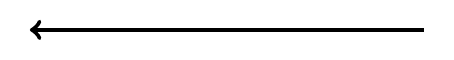
\begin{tikzpicture}
\draw<19-> [ultra thick][->] (5,-5) -- (0,-5);
\end{tikzpicture}

\onslide<19> \textbf{Topological Ordering}

\end{frame}

\begin{frame}{Simulation: Kosaraju's Algorithm (Continued)}

\begin{columns}

\column{0.6\textwidth}

\begin{itemize}
    \item <1> \textbf{Step 2:} Reverse the edges and repeat DFS from topologically sorted nodes
    % \item <2-11> \textbf{Step 3:} Repeat the DFS 
    % \item <12> \textbf{All Strongly Connected Components Found!}
\end{itemize}

\begin{figure}[t]
\begin{tikzpicture}


\node<1-6>[Node] (A_Node) {A};
\node<2-6>[Node_2] (A_Node) {A};
\node<1-6>[Node] (B_Node) [below of=A_Node,yshift = -5mm] {B};
\node<3-6>[Node_2] (B_Node) [below of=A_Node,yshift = -5mm] {B};
\node<1-6>[Node] (C_Node) [right of=A_Node,xshift = 5mm] {C};
\node<5-6>[Node_2] (C_Node) [right of=A_Node,xshift = 5mm] {C};
\node<1-6>[Node] (D_Node) [below of=C_Node,yshift = -5mm] {D};
\node<4-6>[Node_2] (D_Node) [below of=C_Node,yshift = -5mm] {D};


\node<1-10>[Node] (E_Node) [right of=D_Node,xshift = 5mm] {E};
\node<7-10>[Node_2] (E_Node) [right of=D_Node,xshift = 5mm] {E};
\node<1-10>[Node] (F_Node) [right of=E_Node,xshift = 5mm] {F};
\node<8-10>[Node_2] (F_Node) [right of=E_Node,xshift = 5mm] {F};
\node<1-10>[Node] (G_Node) [above of=E_Node,yshift = 5mm,xshift = 5mm] {G};
\node<9-10>[Node_2] (G_Node) [above of=E_Node,yshift = 5mm,xshift = 5mm] {G};

\node<1-12>[Node] (H_Node) [right of=F_Node,xshift = 5mm] {H};
\node<11-12>[Node_2] (H_Node) [right of=F_Node,xshift = 5mm] {H};



\draw<1-6> [->,ultra thick] (C_Node) to (A_Node);
\draw<1-6> [->,ultra thick] (A_Node) to (B_Node);
\draw<1-6> [->,ultra thick] (B_Node) to (D_Node);
\draw<1-6> [->,ultra thick] (D_Node) to (C_Node);
\draw<1-6> [->,ultra thick] (E_Node) to (D_Node);
\draw<1-10> [->,ultra thick] (E_Node) to (F_Node);
\draw<1-10> [->,ultra thick] (H_Node) to (F_Node);
\draw<1-10> [->,ultra thick] (G_Node) to (E_Node);
\draw<1-10> [->,ultra thick] (F_Node) to (G_Node);


    \draw <6> [blue][dashed,ultra thick] (0.75,-0.8) circle [radius=1.55];
    \draw <10> [blue][dashed,ultra thick] (3.65,-0.8) circle [radius=1.55];
    % \draw <12> [blue][dashed,ultra thick] (6.0,-1.5) circle [radius=0.8];



\end{tikzpicture}
\end{figure}



\column{0.3\textwidth}

\centering
Strongly Connected Components


\begin{figure}[t]
\begin{tikzpicture}

\node<6->[Node] (A_Node) {A};
\node<6->[Node] (B_Node) [below of=A_Node,yshift = -5mm] {B};
\node<6->[Node] (C_Node) [right of=A_Node,xshift = 5mm] {C};
\node<6->[Node] (D_Node) [below of=C_Node,yshift = -5mm] {D};


\draw<6-> [->,ultra thick] (A_Node) to (C_Node);
\draw<6-> [->,ultra thick] (B_Node) to (A_Node);
\draw<6-> [->,ultra thick] (D_Node) to (B_Node);
\draw<6-> [->,ultra thick] (C_Node) to (D_Node);

\end{tikzpicture}
\end{figure}

\begin{figure}[t]

\begin{tikzpicture}

\node<10->[Node] (E_Node) {E};
\node<10->[Node] (F_Node) [right of=E_Node,xshift = 5mm] {F};
\node<10->[Node] (G_Node) [above of=E_Node,yshift = 5mm,xshift = 5mm] {G};

\draw<10-> [->,ultra thick] (F_Node) to (E_Node);
\draw<10-> [->,ultra thick] (E_Node) to (G_Node);
\draw<10-> [->,ultra thick] (G_Node) to (F_Node);

\end{tikzpicture}
\end{figure}


\column{0.1\textwidth}

\begin{figure}[t]

\begin{tikzpicture}

\node<12->[Node] (H_Node) {H};


\end{tikzpicture}
\end{figure}



\end{columns}


\centering
\textbf{Stack}
\begin{tabular}{|c|c|c|c|c|c|c|c|}
     \onslide<1-11> B & \onslide<1-10> H & \onslide<1-8> F & \onslide<1-8> G & \onslide<1-6> E & \onslide<1-5> C & \onslide<1-5> D & \onslide<1> A \\
\end{tabular}

\end{frame}

\begin{frame}{Applications}
    
    \begin{itemize}
        \item <1-> Directed Acyclic Subgraph Formation
        \item <2-> Social Connectivity Network Analysis
        \item <3-> Map Processing and Vehicle Routing
    \end{itemize}
    
\end{frame}

\appendix

\begin{frame}{Thank You}
\centering
    \large{Any Questions?}
\end{frame}

\end{document}

%FRAME AND FIGURE
% \begin{frame}{Frame 1}
% This is some text in the first frame. 
% \end{frame}

% \begin{frame}{Frame 2}
% \begin{figure}[h]
% 	\centering
% 	\caption{This caption is at the top}
% 	\includegraphics[scale=0.4]{graph.png}
% 	\label{fig:1}
% 	%\caption{This is figure 1.}
% \end{figure}
% \end{frame}
